%%%%%%%%%%%%%%%%%
% This is an example CV created using altacv.cls (v1.3, 10 May 2020) written by
% LianTze Lim (liantze@gmail.com), based on the
% Cv created by BusinessInsider at http://www.businessinsider.my/a-sample-resume-for-marissa-mayer-2016-7/?r=US&IR=T
%
%% It may be distributed and/or modified under the
%% conditions of the LaTeX Project Public License, either version 1.3
%% of this license or (at your option) any later version.
%% The latest version of this license is in
%%    http://www.latex-project.org/lppl.txt
%% and version 1.3 or later is part of all distributions of LaTeX
%% version 2003/12/01 or later.
%%%%%%%%%%%%%%%%

%% If you are using \orcid or academicons
%% icons, make sure you have the academicons
%% option here, and compile with XeLaTeX
%% or LuaLaTeX.
% \documentclass[10pt,a4paper,academicons]{altacv}

%% Use the "normalphoto" option if you want a normal photo instead of cropped to a circle
% \documentclass[10pt,a4paper,normalphoto]{altacv}

\documentclass[10pt,a4paper,ragged2e,withhyper]{altacv}

%% AltaCV uses the fontawesome5 and academicon fonts
%% and packages.
%% See http://texdoc.net/pkg/fontawesome5 and http://texdoc.net/pkg/academicons for full list of symbols. You MUST compile with XeLaTeX or LuaLaTeX if you want to use academicons.

% Change the page layout if you need to
\geometry{left=1.25cm,
right=1.25cm,
top=1.5cm,
bottom=1.5cm,
columnsep=1.2cm}

% The paracol package lets you typeset columns of text in parallel
\usepackage{paracol}

% include background
\usepackage[scale=10,angle=0,opacity=0.5]{background}
\backgroundsetup{contents={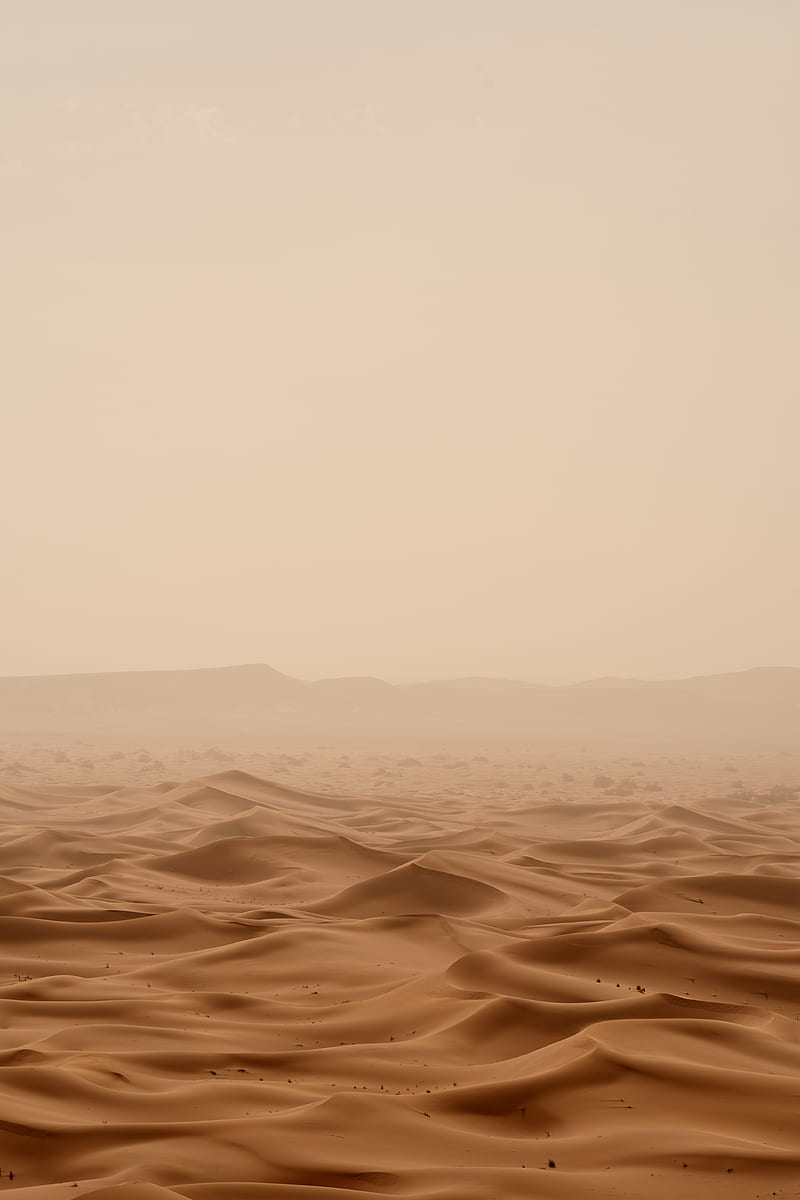
\includegraphics[width=.15\textwidth]{HD-wallpaper-desert-under-white-sky-during-daytime.jpg}}}

% Change the font if you want to, depending on whether
% you're using pdflatex or xelatex/lualatex
\ifxetexorluatex
  % If using xelatex or lualatex:
  \setmainfont{Lato}
\else
  % If using pdflatex:
  \usepackage[default]{lato}
\fi

% Change the colours if you want to

\definecolor{White}{HTML}{ffffff}
\definecolor{RedBullYellow}{HTML}{ffd300}
\definecolor{RedBullWhite}{HTML}{f4ebee}
\definecolor{RedBullGray}{HTML}{d9d4ce}
\definecolor{RedBullRed}{HTML}{e21b4d}

\definecolor{UAEGreen}{HTML}{007F3F} % Green from the UAE flag
\definecolor{UAEWhite}{HTML}{FFFFFF} % White from the UAE flag
\definecolor{UAERed}{HTML}{EF3340}   % Red from the UAE flag
\definecolor{UAEBlack}{HTML}{000000} % Black from the UAE flag

% Define UQ colors
\definecolor{UQPurple}{HTML}{51247A}  % UQ Purple
\definecolor{UQGold}{HTML}{FFB81C}    % UQ Gold
\definecolor{UQDarkGray}{HTML}{4C4C4C} % UQ Dark Gray
\definecolor{UQLightGray}{HTML}{CCCCCC} % UQ Light Gray

\definecolor{DarkYellow}{HTML}{ffcc00}
\definecolor{DarkWhite}{HTML}{f2f2f2}
\definecolor{VividPurple}{HTML}{3E0097}
\definecolor{DodgerBlue}{HTML}{338DFF}
\definecolor{MediumTurquoise}{HTML}{48D1CC}
\definecolor{DarkBlue}{HTML}{000A8E}
\definecolor{SlateGrey}{HTML}{2E2E2E}
\definecolor{LightGrey}{HTML}{666666}

\colorlet{name}{UAEGreen}
\colorlet{tagline}{UAEBlack}
\colorlet{heading}{UAEBlack}
\colorlet{headingrule}{UAEBlack}
\colorlet{subheading}{UAEBlack}
\colorlet{accent}{UQPurple}
\colorlet{emphasis}{UAEBlack}
\colorlet{body}{UAEBlack}
\usepackage{xcolor} % Add this in your preamble

% Change some fonts, if necessary
% \renewcommand{\namefont}{\Huge\rmfamily\bfseries}
% \renewcommand{\personalinfofont}{\footnotesize}
% \renewcommand{\cvsectionfont}{\LARGE\rmfamily\bfseries}
% \renewcommand{\cvsubsectionfont}{\large\bfseries}

% Change the bullets for itemize and rating marker
% for \cvskill if you want to
\renewcommand{\itemmarker}{{\small\textbullet}}
\renewcommand{\ratingmarker}{\faCircle}

%% sample.bib contains your publications
\addbibresource{sample.bib}

\begin{document}
\name{Andrea Zignoli}
\tagline{M.Eng, PhD | Applied Research Scientist \& Consultant in Sport Technology}
% Cropped to square from https://en.wikipedia.org/wiki/Marissa_Mayer#/media/File:Marissa_Mayer_May_2014_(cropped).jpg, CC-BY 2.0
%% You can add multiple photos on the left or right
\photoR{2.5cm}{profile_pic_1_1}
% \photoL{2cm}{Yacht_High,Suitcase_High}
\personalinfo{%
  % Not all of these are required!
  % You can add your own with \printinfo{symbol}{detail}
  \email{andrea.zignoli@unitn.it}
%   \phone{000-00-0000}
  \mailaddress{Via Barbassa, 37029, Verona}
  \location{Italy}\\
  \homepage{andreazignoli.github.io/}
  \twitter{@andrea_zignoli}
  \linkedin{andrea-zignoli-8080a438}
  \researchgate{Andrea-Zignoli}
 \github{andreazignoli} % I'm just making this up though.
%   \orcid{orcid.org/0000-0000-0000-0000} % Obviously making this up too. If you want to use this field (and also other academicons symbols), add "academicons" option to \documentclass{altacv}
  %% You MUST add the academicons option to \documentclass, then compile with LuaLaTeX or XeLaTeX, if you want to use \orcid or other academicons commands.
  % \orcid{0000-0000-0000-0000}
  %% You can add your own arbtrary detail with
  %% \printinfo{symbol}{detail}[optional hyperlink prefix]
  % \printinfo{\faPaw}{Hey ho!}
  %% Or you can declare your own field with
  %% \NewInfoFiled{fieldname}{symbol}[optional hyperlink prefix] and use it:
  % \NewInfoField{Research Gate}{\faresearchgate}[Andrea_Zignoli]
  % \gitlab{your_id}
}

\makecvheader

%% Depending on your tastes, you may want to make fonts of itemize environments slightly smaller
\AtBeginEnvironment{itemize}{\small}

%% Set the left/right column width ratio to 6:4.
\columnratio{0.6}

% Start a 2-column paracol. Both the left and right columns will automatically
% break across pages if things get too long.
\begin{paracol}{2}

\cvsection{Presentation}

I'm an applied research scientist with 10+ years of experience developing AI-driven solutions for sports performance analysis, combining academic rigor with real-world impact. 

\cvsection{Current positions}

\cvevent{Applied Research Scientist - Product Expert}{Athletica Inc.}{Apr 2020 -- Ongoing}{Remote location}
\begin{itemize}
\item Part-time back-end lead and product expert. 
\item Responsible for the development of the data processing \& analysis for a web-based endurance training platform. 
\end{itemize}

\divider

\cvevent{Consultant}{Tymewear}{November 2024 -- Ongoing}{Remote location}
\begin{itemize}
\item AI features development - ML models - back-end development. 
\end{itemize}

\divider

\cvevent{Consultant}{Enhance-d}{June 2024 -- Ongoing}{Remote location}
\begin{itemize}
\item Development of DL models from sport-wearable data sources. 
\end{itemize}

% \begin{itemize}
% \item Joined the company as employe \#20 and female employee \#1
% \item Developed targeted advertisement in order to use user's search queries and show them related ads
% \end{itemize}

\cvsection{Stack I use}

\cvachievement{\faCode}{Machine Learning Development}{Python: Scikit Learn - Pandas - Keras - Tensorflow}
\divider\\
\cvachievement{\faShip}{Containerization \& Backend Development}{Docker | Python: Flask | Shiny (R)}
\divider\\
\cvachievement{\faCloud}{Cloud Deployment}{Heroku | AWS Lightsails}

\cvsection{How I spend my time}

% Adapted from @Jake's answer from http://tex.stackexchange.com/a/82729/226
% \wheelchart{outer radius}{inner radius}{
% comma-separated list of value/text width/color/detail}
% Some ad-hoc tweaking to adjust the labels so that they don't overlap
\hspace*{-2cm}  %% quick hack to move the wheelchart a bit left
\wheelchart{1.5cm}{0.5cm}{%
  5/8em/accent!0/Communication \& reporting of results,
  35/13em/accent!250/Time-series analysis,
  30/9em/accent!60/Statistics \& machine learning,
  10/11em/accent!500/Grant writing \& funding,
  15/8em/accent!20/Scientific writing,
  5/9em/accent!120/Data collection
}

% use ONLY \newpage if you want to force a page break for
% ONLY the currentc column
\newpage

\cvsection{Working experience}

\cvevent{Teaching Fellow}{Department of Cellular, Computational and Integrative Biology - CIBIO, University of Trento}{Dec 2021 -- Ongoing}{Trento, I}
\begin{itemize}
\item Instructor for the 3-credit module on Modeling within the Technology and Innovation in Sports course in the Master’s program in Exercise Science and Human Movement
\end{itemize}

\divider

\cvevent{Fellow Researcher}{Department of Industrial Engineering, University of Trento}{Dec 2020 -- Ongoing}{Trento, I}
\begin{itemize}
\item Development and deployment of mathematical models for sport technology applications.
\end{itemize}

\divider

\cvevent{Associate Editor}{Sports Engineering, the official journal of the International Sports Engineering Association (ISEA)}{Oct 2021 -- Ongoing}{Remote location}

\begin{itemize}
\item Handling and reviewing research papers. 
\item Creating partnerships with sport tech companies, governing bodies, and organising committees. 
\end{itemize}

\divider

\cvevent{Applied Research Scientist}{Supersapiens}{Apr 2020 -- Apr 2024}{Remote location}
\begin{itemize}
\item Data analysis and report creation (internal, coaches, athletes, users)
\item Product design and scientific support
\end{itemize}

\divider

\cvevent{Functional evaluation centre}{CeRiSM Sport Mountain and Health Research Centre}{Apr 2012 -- Oct 2017}{Trento, I}
\begin{itemize}
\item Data collection and athlete functional evaluation
\item Scientific writing
\end{itemize}

\cvsection{Key Publications}

\nocite{*}

%\printbibliography[heading=pubtype,title={\printinfo{\faBook}{Books}},type=book]

%\divider

\printbibliography[heading=pubtype,title={\printinfo{\faFile*[regular]}{Journal Articles (selection)}}, type=article]

\divider

\printbibliography[heading=pubtype,title={\printinfo{\faUsers}{Conference Proceedings (selection)}},type=inproceedings]

%% Switch to the right column. This will now automatically move to the second
%% page if the content is too long.
\switchcolumn

\cvsection{Education}

\cvevent{PhD\ in Science of Physical Exercise and Human Movement}{University of Verona, Verona, Italy}{Jan 2013 -- May 2016}{}

\divider

\cvevent{M.Eng.\ in Mechatronics}{University of Trento, Trento, Italy}{Sept 2008 -- March 2011}{}


\cvsection{Metrics \tiny{(Scopus)}}

\cvachievement{\faTasks}{43 peer-reviewed publications}{41\% first-author | 8\% single-author}

\divider

\cvachievement{\faProjectDiagram}{329 Citations (H-index 10)}{20.5\% (8 documents) in the top 25\% most cited documents worldwide}

\cvsection{Coding Skills}

\cvtag{Python} \cvtag{R} \cvtag{Matlab} 

\cvsection{Statistics \& ML}

\cvtag{(RM)-ANOVA} \cvtag{Multi-linear models}\\
\cvtag{PCA} \cvtag{SVM}\\
\cvtag{Deep learning} \\
\cvtag{CNN} \cvtag{LSTM} \cvtag{GAN}

\cvsection{Data processing}

\cvtag{GPS} \cvtag{Power meters} \cvtag{EMG} \cvtag{NIRS} \\ 
\cvtag{Lactate monitors} \cvtag{Pressure insoles} \\
\cvtag{CPET} \cvtag{IMU} \cvtag{Motion capture} \\
\cvtag{Force platforms} \cvtag{Optitrack} \cvtag{HRV}  \\

\cvsection{Languages}

\cvskill{Italian}{5}
% \divider
\cvskill{English}{4}
% \divider

\newpage

\cvsection{Side Projects I lead}

\cvachievement{\faLungs}{Oxynet}{\href{https://www.oxynet.net}{\textcolor{blue}{www.oxynet.net}}}  
Process and interpret cardiopulmonary exercise tests with AI technologies.  

\divider  

\cvachievement{\faBatteryHalf}{Workout Reserve}{\href{https://andreazignoli.github.io/athletica-workout-reserve/}{\textcolor{blue}{github.io}}}  
The Athletica Workout Reserve Connect IQ App for endurance athletes.

\divider  

\cvachievement{\faBicycle}{CURVA}{\href{https://bitbucket.org/andrea_zignoli/optimal-itt/src/master/}{\textcolor{blue}{bitbucket.org}}}  
Cycling trajectories optimized using optimal control.  

\divider  

\cvachievement{\faHelicopter}{Drone Footage}{\href{https://github.com/andreazignoli/drone_footage}{\textcolor{blue}{github.com}}}  
Processing and analysis of drone footage for cycling applications.  

\divider  

\cvachievement{\faRunning}{PRISSV}{\href{https://bitbucket.org/andrea_zignoli/prissiv/src/np/}{\textcolor{blue}{bitbucket.org}}}  
Running step frequency analysis using IMUs and deep learning models.  

\cvsection{Referees}

\cvref{Prof.\ Paul B. Laursen}{HIIT Science}{paul@hiitscience.com}
{1311 Lee Road, \\
Revelstoke, B.C., Canada}

\divider

% \cvref{name}{email}{mailing address}
\cvref{Prof.\ Francesco Biral}{University of Trento}{francesco.biral@unitn.it}
{Via Sommarive 9, 38123\\Trento, Italy}

\end{paracol}

\end{document}
